\documentclass{article}

\usepackage[utf8]{inputenc}
%\usepackage{medievalunicodefont}
\usepackage{ebgaramond}

\usepackage{graphicx} % Required for inserting images
\usepackage{hyperref}
\usepackage{url}

\usepackage[english, french]{babel}

\usepackage{setspace}

\usepackage{hyperref}

\usepackage{enumitem}

\date{}


\title{Séminaire \og Fondamentaux Informatiques: Git\fg \\ Master 1 - 2022-2023\\ \large
M. Jean-Victor Boby \\ \small Lise Bernard, Axël Le Boulicaut, Charlie Lézin, Axelle Salvador \\ Lien vers le projet : \url{https://github.com/asalva15/HN-2022--PROJET-DU-GUESCLIN--}}



\begin{document}

\maketitle
\begin{figure}[ht]
  \centering
  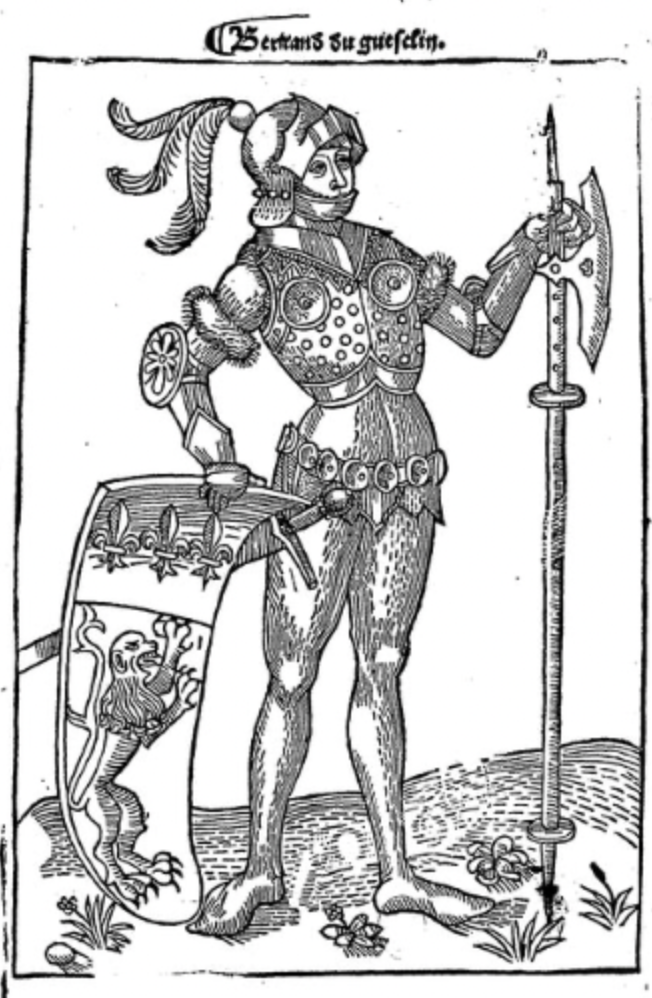
\includegraphics[width=6.5cm]{Bertrand.png}
  \caption{\small Bertrand du Guesclin, \textit{Le Livre des faits de messire Bertrand du Guesclin}, 1487, p. 1}
\end{figure}


\includegraphics[width=3cm]{Unknown.png}

\setstretch{1.3}


\section{Introduction}

Notre projet se concentre sur \textit{Le Livre des faits de messire Bertrand du Guesclin}, plus précisément sur une édition de 1487, disponible en ligne sur Gallica\footnote{En suivant ce lien : \url{https://gallica.bnf.fr/ark:/12148/bpt6k1110614/f5.item}} - il est consultable à la Bibliothèque nationale de France\footnote{La notice de l'ouvrage dans le catalogue de la BNF est la suivante : \url{https://catalogue.bnf.fr/ark:/12148/cb33258730z}} -, en caroline gothique, le texte est imprimé.\\

	Bertrand du Guesclin est né vers 1320 au château de la Motte-Broons près de Dinan. 
Bertrand est le fils aîné de Robert II Du Guesclin et de Jeanne de Malesmains, dame de Sens-de-Bretagne. Très jeune il part vivre chez son oncle, Bertrand Du Guesclin seigneur de Vauruzé près de Rennes. Selon les chroniques de l'époque, il participe à son premier tournoi le 4 juin 1337 et défait une quinzaine de chevaliers. La guerre de cent ans lui permet également d’obtenir la reconnaissance d’une partie de la noblesse en se faisant adouber en 1357. Il est nommé capitaine de Pontorson et du mont Saint-Michel. En 1360 il est nommé lieutenant de Normandie, d’Anjou et du Maine et en 1364 capitaine général pour les pays entre Seine et Loire et chambellan de France. Du Guesclin s’illustre la même année à Cocherel en remportant une bataille contre Charles II de Navarre. Durant la guerre de succession de Bretagne, il prend le parti de Charles de Blois qui s’oppose à Jean de Montfort. Son armée est défaite à Auray et il est fait prisonnier par les anglais, le roi de France paie alors une rançon de 100 000 livres pour sa libération. À sa libération, Charles V le fait connétable de France, il reconquiert ainsi la Normandie, la Guyenne, la Saintonge et le Poitou. Il meurt le 13 juillet 1380 à Châteauneuf-de-Randon.\\ 

Le passage que nous avons transcrit sur situe au tout début de l’ouvrage, et occupe les folios un (carré noir) à neuf (\og fort \fg\hspace{0.5mm}), soit seize colonnes.


\section{Présentation des données sources}

\subsection{La Chronique abrégée de Bertrand Du Guesclin}

La vie de Bertrand Du Guesclin est un texte imprimé publié en 1487 par Guillaume Le Roy, l’imprimeur et libraire à Lyon à la fin du XVème siècle. Son auteur est anonyme. Le livre est divisé en trois partie, on trouve tout d'abord une introduction avec une présentation de Bertrand Du Guesclin et du contexte historique. La première partie est consacrée aux exploits de Bertrand Du Guesclin en Bretagne, la deuxième partie est consacrée aux batailles que Bertrand Du Guesclin à mené en Espagne. Enfin, la troisième partie relate la fin de sa vie. Cette chronique médiévale permet une meilleure compréhension du XIVème siècle et plus particulièrement de la guerre de Cent ans. On voit également, à travers le personnage de Bertrand Du Guesclin, la vie d'un seigneur breton de l'époque, son entourage, son quotidien et ses obligations vis à vis de son suzerain le roi de France. C'est également une source très précieuse dans le domaine de la littérature médiévale. 

\setlength{\parskip}{0.5cm}

Cet ouvrage est composé de 88 folios relatant la vie et les exploits de Bertrand Du Guesclin. Les folios sont rédigés en français moyen et en lettres gothiques. 

\setlength{\parskip}{0.5cm}

Il est aujourd’hui conservé à la Bibliothèque nationale de France. À l’origine cette chronique abrégée fait partie d’un ouvrage intitulé \textit{Le Triumphe des neuf preux}\footnote{Que l’on peut consulter en suivant ce lien : \url{https://www.persee.fr/doc/shf_0000-0000_1904_num_4_1_953_t1_0070_0000_2/}}.

\section{Ontologie et normes de transcription}

\subsection{Normes de transcription}

Nos normes de transcription sont explicitées sur un fichier en \textit{markdown} de notre dépôt github. La majorité des choix de transcription ont été discutés sur les issues ou ont suivi le guide paléographique d'Ariane Pinche.\footnote{Que l’on peut consulter en suivant ce lien : \url{https://hal.science/hal-03697382/}}. \\

Les paragraphes sont indiqués dans notre monographie imprimée par des pieds de mouche noirs ; ils ont été transcrits par le caractère \og ¶ \fg\hspace{0.5mm}. 

Notre monographie contient plusieurs lettres ramistes, notamment les \og u \fg et les \og v \fg, ainsi que les \og i \fg et les \og j \fg. Cela signifie qu'à l'intérieur des mots, les lettres \og u \fg\hspace{0.5mm}  et \og v \fg\hspace{0.5mm} sont indistinctes. En position initiale, le \og u \fg\hspace{0.5mm}  et le \og v \fg\hspace{0.5mm}  prennent la même valeur, avec une forme particulière que nous avons choisi de distinguer. Prenons un exemple, la première lettre du mot \og ueoir \fg\hspace{0.5mm} sera indiquée par un signe qui ressemble à un b minuscule en cyrillique (voir le fichier normes de transcriptions). De même, en position initiale, les caractères ayant valeur de \og i \fg\hspace{0.5mm}  ou \og j \fg\hspace{0.5mm}  suivent la même graphie, comme avec \og iehan \fg\hspace{0.5mm}  pour \og jehan \fg\hspace{0.5mm}. 

Nous avons choisi de représenter la distinction entre les \og s \fg\hspace{0.5mm}  longs et les \og s \fg\hspace{0.5mm}  ronds. 

Le \og b \fg\hspace{0.5mm}  prend deux graphies dans le texte, une avec une barre droite et l'autre avec une boucle. Nous avons choisi de garder une seule graphie pour représenter ces deux lettres : \og b \fg\hspace{0.5mm} (avec une barre droite). D'ailleurs, nous avions d'abord opté pour une lettre qui revient à un \og g \fg\hspace{0.5mm} à l'envers pour représenté le b avec une boucle, mais qui ne convenait pas parce qu'elle se situait en-deçà des autres lettres sur la ligne. 

Le \og d \fg\hspace{0.5mm}, quant à lui, a une graphie particulière dans le texte que nous avons choisi de signaler par un signe qui ressemble à une esperluette à l'envers. 

Le  \og r \fg\hspace{0.5mm} prend deux graphies dans notre texte, nous avons là aussi choisi de distinguer sa variation \og rotunda \fg\hspace{0.5mm}, utilisé quand le \og r \fg\hspace{0.5mm} suit une lettre arrondie, sinon on utilise le \og r \fg\hspace{0.5mm} que l'on connaît. 

Le \og z \fg\hspace{0.5mm} prend lui aussi une graphie particulière dans notre texte : nous avons choisi d'indiquer cette variation, en utilisant un caractère ressemblant à un \og 3 \fg\hspace{0.5mm}.\\

Les mots sont séparés de manière claire dans le texte, nous avons donc suivi cela. Dans certains cas, une césure est marquée par un trait de suite, noté par une diagonale de gauche à droite. Nous avons donc utilisé un trait penché dans cette direction pour le représenter dans notre transcription.\\

De plus, les abréviations présentes dans le texte ont été conservées. Pour cela, nous nous sommes appuyés sur un article reprenant les abréviations paléographique, proposé par le \textit{Carnet de l'Institut de Recherche et d'Histoire des Textes}\footnote{Disponible sur le lien suivant : \url{https://irht.hypotheses.org/792}}. Ainsi, différents signes spéciaux ou certaines lettres sont utilisés pour représenter un ensemble de lettres. 

Les lettres \og pro \fg\hspace{0.5mm} sont représentées par un p dont la barre est bouclée. Dans notre cas, ce signe apparaît pour le mot  \og prochain \fg\hspace{0.5mm}. Les lettres \og ou \fg ou \og ous \fg ont elles aussi une graphie spécifique.

Le q tilde est largement utilisé dans notre texte en tant qu'abréviation de \og que \fg\hspace{0.5mm} ou \og qu' \fg\hspace{0.5mm}. Le tilde est beaucoup utilisé dans le texte. Représenté par un trait droit proche du macron, nous avons décidé conserver le tilde, présente sur toutes les voyelles (sauf y).

Le nom de Bertrand du Guesclin est lui aussi parfois abrégé. Ainsi, il peut être indiqué par un \og b \fg\hspace{0.5mm} minuscule entre deux points ou par un \og B \fg\hspace{0.5mm} majuscule entre deux points.

Nous avons suivi la ponctuation présente dans la monographie imprimée. Elle est notamment indicative des abréviations et des chiffres, comme nous l'avons indiqué pour le le nom de Bertrand du Guesclin. Les chiffres aussi sont encadrés par deux points, qu'ils soient écrits en lettres ou en chiffres romains.

\subsection{Ontologie}

Le mot \og ontologie \fg\hspace{0.5mm} est défini comme tel dans un article de Dominique Stutzmann comme une \og description formelle de la réalité et des relations entre concepts, répartissant les objets et les concepts (« individus ») en différentes classes subordonnées ou associées les unes aux autres, et définies par leurs attributs et leurs relations \fg\footnote{Dominique Stutzmann, « Ontologie des formes et encodage des textes manuscrits médiévaux. Le projet ORIFLAMMS », \textit{Document numérique}, vol. 16, no. 3, 2013, pp. 81-95, URL : \url{https://www.cairn.info/revue-document-numerique-2013-3-page-81.htm\#no1}}. 

Si plusieurs catégories sont déjà disponibles sur le logiciel eScriptorium (\textit{Commentary, Illustration, Main, Title} ou \textit{text}), nous avons ajouté à son ontologie par défaut une \og \textit{region type} \fg\hspace{0.5mm} (une catégorie) que nous avons appelée  \og Colonne / \textit{column}\fg\hspace{0.5mm}, car notre texte se présentait sous cette forme (deux colonnes de texte, cela nous a d'ailleurs posé des problèmes pour la numérotation des lignes). Notons que pour les lignes, nous avons sélectionné les paramètres par défaut, notamment pour les indications de numéros de page et des signatures. De surcroît, nous avions affaire à des lettrines pour certaines pages, lignes que nous avons nommées \og \textit{DropCapital}\fg. 

\section{Difficultés rencontrées au cours du projet}
La majorité des problèmes rencontrés sont liés à la prise en main du logiciel eScriptorium auquel nous n’étions pas habitués. Par ailleurs, nous ne sommes pas familiers à la paléographie, donc nos choix de transcription ne sont peut-être pas toujours les meilleurs. Nous avons choisi de rester très proches de la graphie du texte. Pour nous aider nous nous sommes appuyé.e.s sur différents documents (voir la bibliographie). 

Nous avons eu beaucoup de difficultés au moment de la segmentation : les lignes étaient créées en double et la technique pour les ordonner n’étant pas toujours fonctionnelle, nous avons fait une grande partie de ce travail manuellement. Ainsi, la majeure partie du temps consacré au projet s’est portée sur la transcription (plus que sur la gestion de GitHub). 

Nous avons aussi passé du temps à choisir les différents caractères pour constituer le clavier. Toutefois avec les possibilités des claviers latins et du MUFI nous avons pu choisir les caractères qui nous semblaient les plus adéquats (toujours d’après nos piètres qualités de paléographes). 

Par ailleurs, le fait de se fréquenter quotidiennement dans le même lieu a rendu un peu artificielle l’utilisation des issues puisque nous nous sommes régulièrement vus pour discuter du projet. 

Sur GitHub, nous avons eu des problèmes au début du projet en créant un repository privé ce qui rendait compliqué toutes les manipulations sur Git. Nous avons donc choisi de laisser le repository public puisque seules des personnes de confiance y avait accès. 
Ensuite, nous avons eu du mal à choisir les branches à merge dans notre projet. En effet, nous avions d’abord créé une branche par personne avec nos premières versions de correction. Finalement, d’un commun accord, nous nous sommes dit qu’il n’était pas nécessaire de les merger. Ainsi, nous sommes allés récupérer les premières versions des autres pour les corriger puis ensuite nous les avons ajoutées dans une nouvelle branche que nous avons merge à la branche principale. Enfin, nous avons fini par organiser la branche main avec l’ensemble des documents. 

Enfin, une difficulté récurrente est la présence de fichier .DS\_Store automatiquement créés dans les dossiers sur macOS (pour l’affichage des éléments). Cependant, même en l’ajoutant à notre .gitignore, nous avons commit plusieurs fois ce type de fichier dans nos branches ce qui n’était pas nécessaire.



\section{Bibliographie}

\subsection{La source}

Voici le lien vers la Chronique abrégée de Bertrand Du Guesclin : 

\setlength{\parskip}{0.5cm}

\href{https://gallica.bnf.fr/ark:/12148/bpt6k1110614/f5.item}{https://gallica.bnf.fr/ark:/12148/bpt6k1110614/f5.item}

\noindent\textbf{Références bibliographiques principales :}

\begin{enumerate}
\item Cuvelier, Johannes. \textit{Chronique de Bertrand Du Guesclin}. Paris : Imprimerie de Béthune et Plon, 1839.
\item Michaud, Louis-Gabriel. \textit{Biographie universelle, ancienne et moderne}. Paris : Madame C. Desplaces, 1842.
\item Jacob, Yves. \textit{Bertrand Du Guesclin connétable de France}. Paris : Fayard, 1992.
\item Minois, Georges. \textit{Du Guesclin}. Paris : Perrin, 1993.
\item Favier, Jean. \textit{La Guerre de Cent ans}. Paris : Fayard, 1980.
\end{enumerate}

\subsection{e-Scriptorium}

Voici le lien vers la page principale d'e-sciptorium : 

\setlength{\parskip}{0.5cm}

\href{https://escriptorium.inria.fr/}{https://escriptorium.inria.fr/}

Voici deux liens vers des pages d'aide pour apprendre à utiliser e-sciptorium:  

\begin{enumerate}
    \item Peter A. Stockes \og eScriptorium : un outil pour la transcription automatique des documents\fg \:\textit{ÉpheNum}. \url{https://ephenum.hypotheses.org/1412}
    \item \og Prendre en main eScriptorium \fg, \textit{LECTAUREP}. \url{https://lectaurep.hypotheses.org/documentation/prendre-en-main-escriptorium}
\end{enumerate}

\subsection{Outil : aide à la transcription du XVème siècle}
\begin{enumerate}
    \item \og Abréviations paléographiques \fg, \textit{Carnets de l'IRHT}. \url{https://irht.hypotheses.org/792}
    \item Ariane Pinche. \textit{Guide de transcription pour les manuscrits du Xe au XVe siècle.} 2022. \url{https://hal.science/hal-03697382/}
    \item Dominique Stutzmann, « Ontologie des formes et encodage des textes manuscrits médiévaux. Le projet ORIFLAMMS », \textit{Document numérique}, vol. 16, no. 3, 2013, pp. 81-95, URL : \url{https://www.cairn.info/revue-document-numerique-2013-3-page-81.htm\#no1}
\end{enumerate}

\end{document}
